\chapter{Le rôle des paysans participant au projet de sélection collaborative sur les céréales}

\begin{center}
\Large Version 5 du 30 septembre 2015
\end{center}


\section{Réunion de bilan de l'année écoulée et des prochains semis}
Cette réunion a lieu dans la deuxième semaine de septembre à Paris. Pour le suivi de la dynamique,
il est important que l'animateur et au moins un paysan y soient présents.

\section{Les semis : dispositifs expérimentaux}


\warning{Envoyez à votre animateur la liste des populations que vous souhaitez semer et il vous
proposera un plan de semis. Ensuite, envoyer le plan définitif à votre animateur. Il vous
enverra alors des étiquettes et des piquets afin de bien identifier vos micros-parcelles.}


Pour le semis, deux choses sont importantes :

\begin{itemize}
\item semer le témoin qui vous sera envoyé si vous ne l'avez pas déjà. A part le témoin, vous
semez ce que vous voulez ! Il est important de conserver les noms des sélections que l'on
vous donne lorsque que vous faites des bouquets de sélection (sous la forme [nom de la
variété]\#[une lettre], par exemple Rouge-de-Bordeaux\#R ou Blanc-de-la-Réole\#E)

\item suivre un dispositif expérimental de type ferme régional \yo{OU} satellites.
Pour les fermes satellites, s'il y a peu de populations, on peut imaginer répéter le témoin une seule fois.
\end{itemize}

Les témoins sont dans les cases noires. Les populations que vous choisissez sont dans les cases
blanches. 
La taille conseillée des micro-parcelles est entre 5 et 10m\up{2}.
 \\


\begin{center}
\begin{tabular}{c c}
Fermes régionales & Fermes satellites \\
\hline
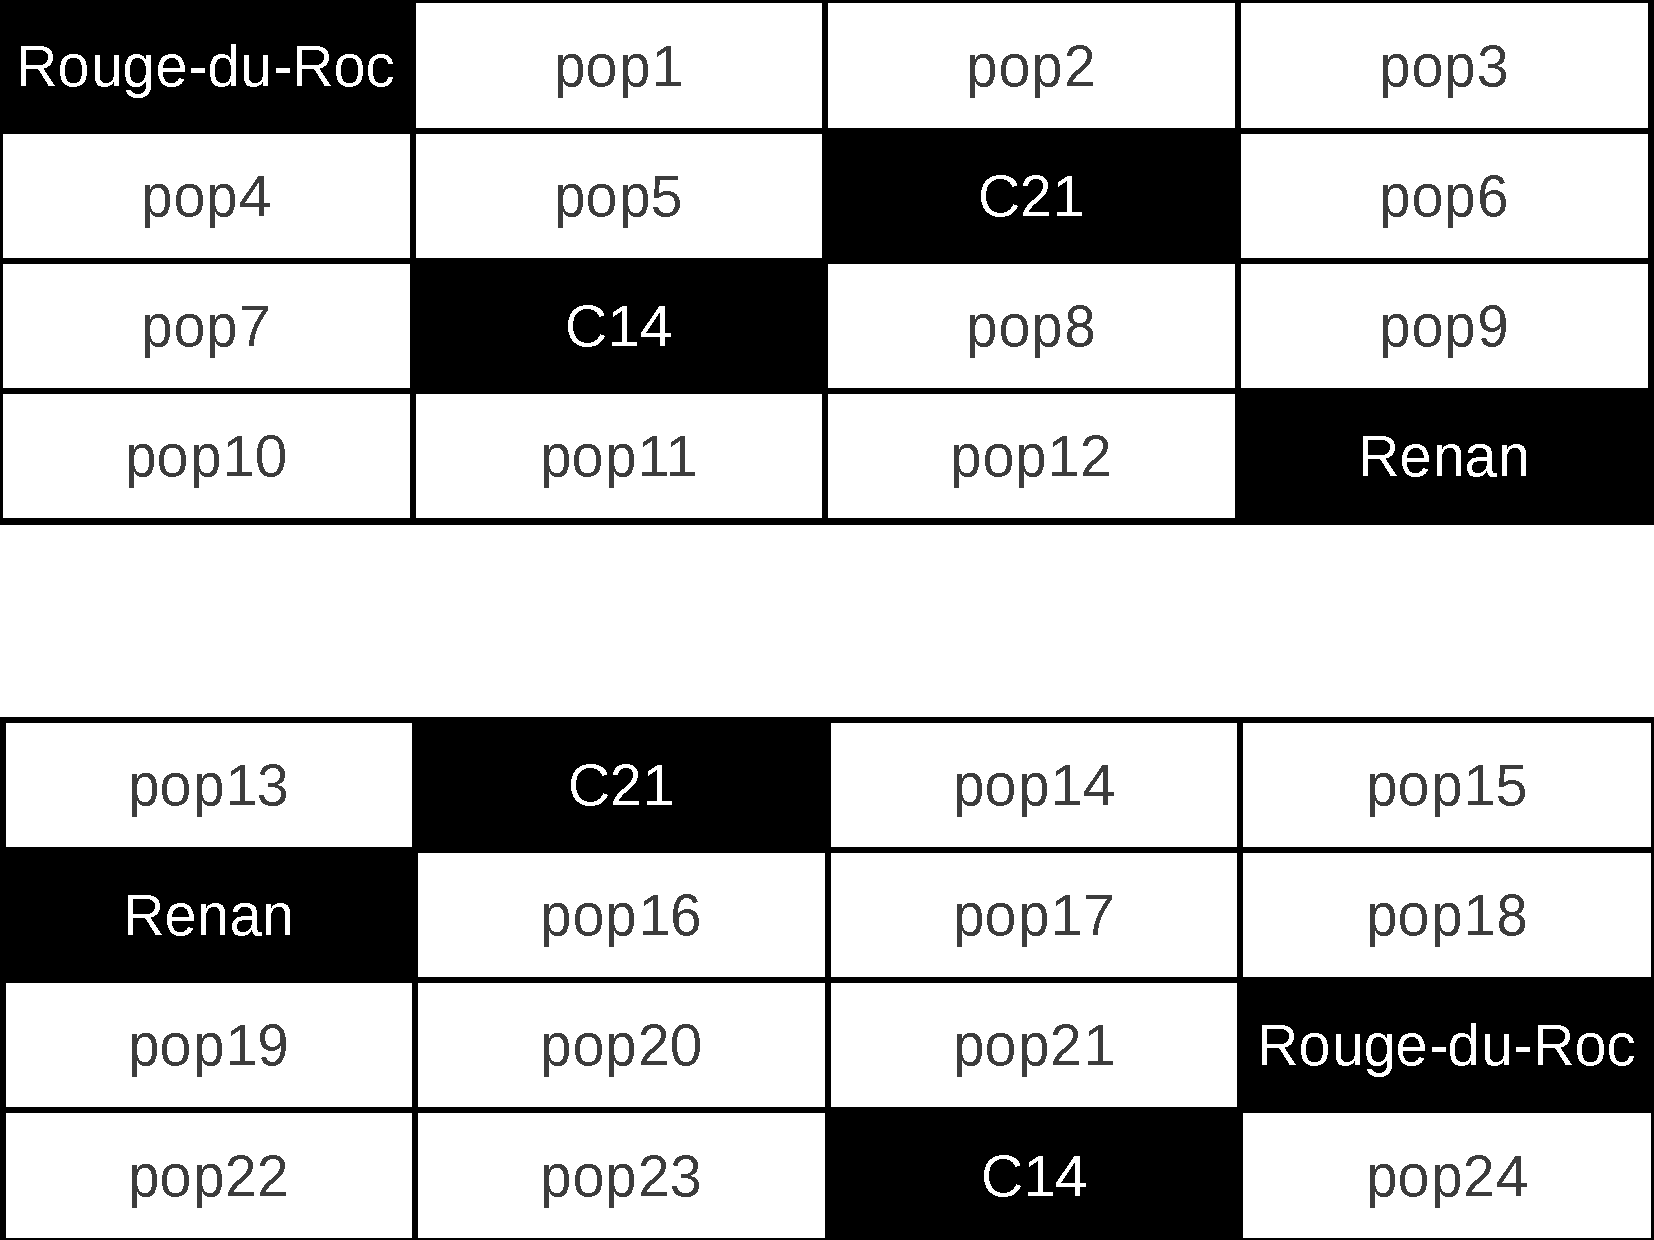
\includegraphics[width=.4\textwidth]{/home/deap/Documents/Gaelle/scriptsR/dossiers_retour/test_dossier_retour/2.tex_files/plan_FR.pdf}  & 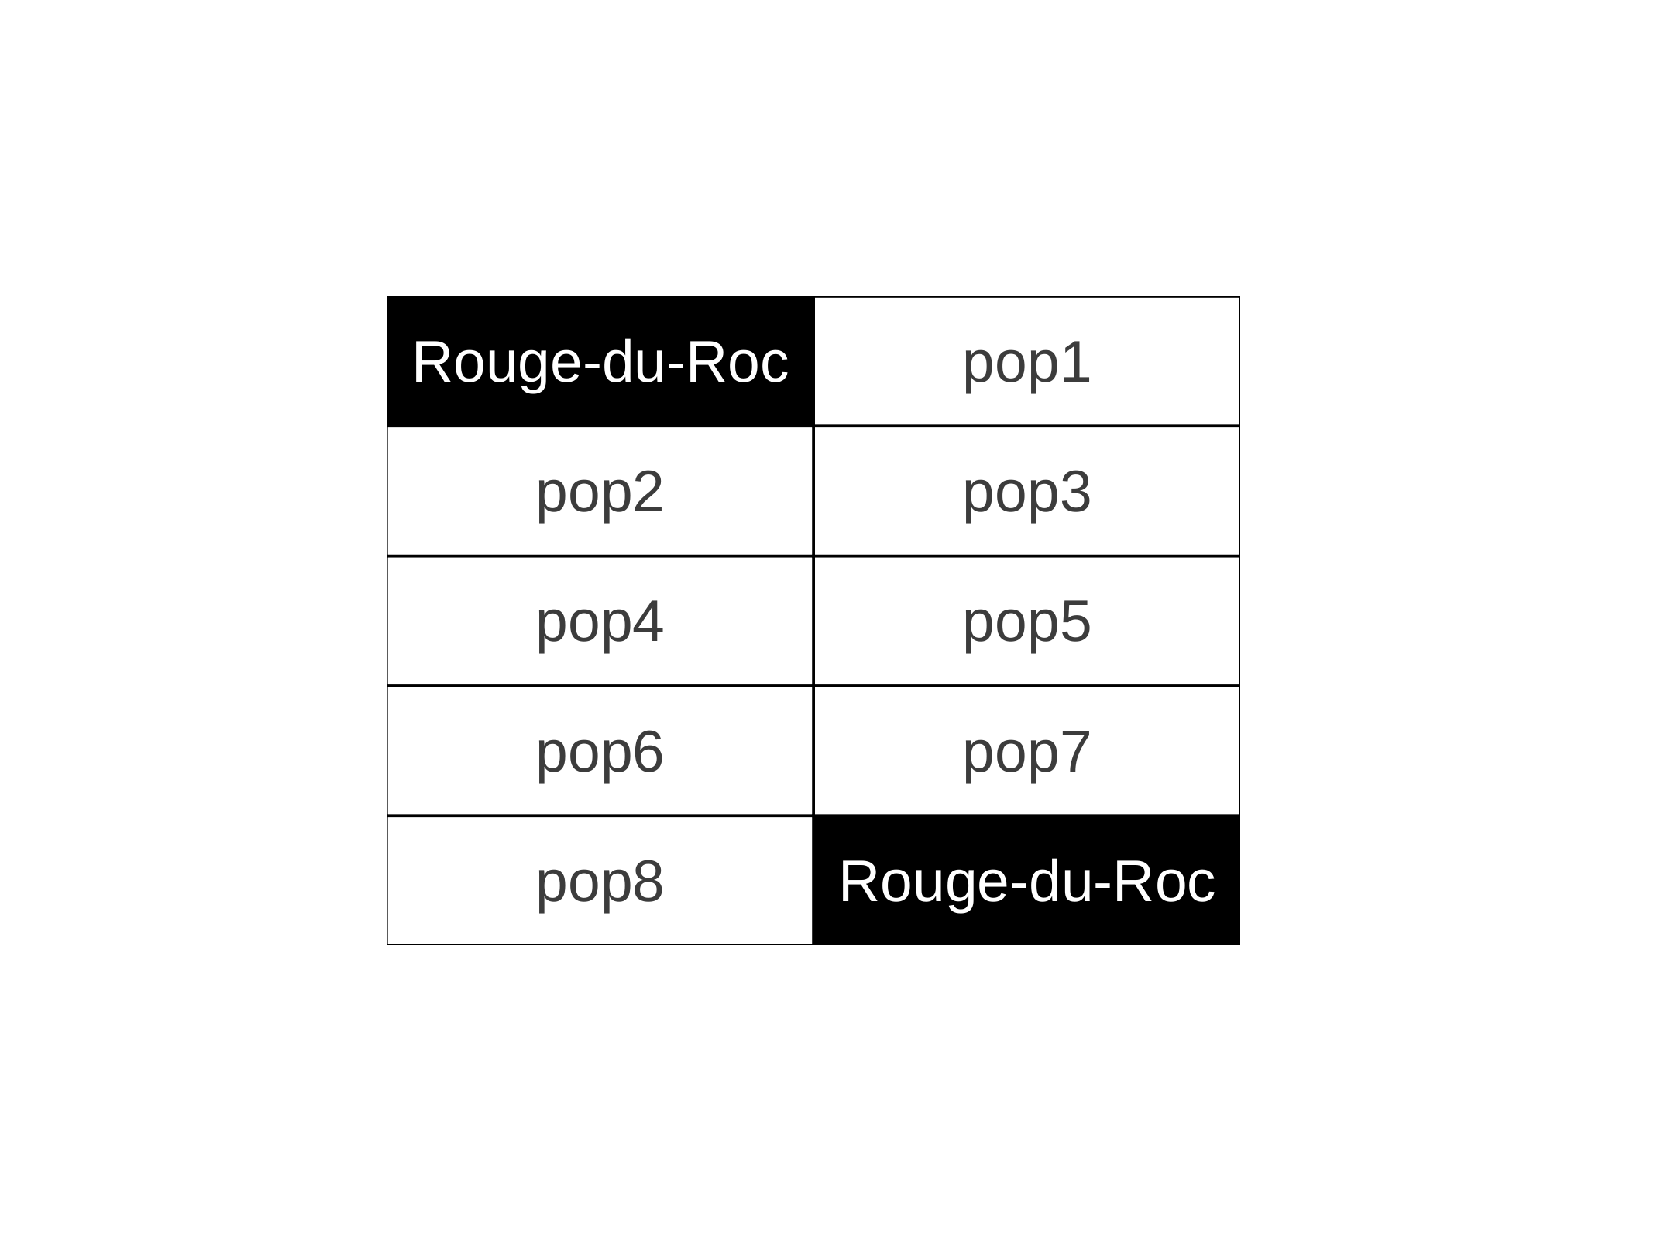
\includegraphics[width=.4\textwidth]{/home/deap/Documents/Gaelle/scriptsR/dossiers_retour/test_dossier_retour/2.tex_files/plan_FS_bis.pdf} 
 \\
\hline
\end{tabular}
\end{center}

\section{Suivi des populations avec les fiches}
Votre animateur vous fera parvenir des fiches afin de suivre la culture. Ces fiches peuvent être
issues du projet national ou issues de votre groupe.

\section{Envoi des épis récoltés par la poste pour qu'ils soient mesurés à l'INRA}

A la récolte, votre animateur vous enverra un courrier avec deux types d'enveloppes :

\begin{itemize}
\item \yo{« 50 épis au hasard »} pour y déposer 50 épis (ou moins s'il y a peu d'épis dans la micro-
parcelle) pris au hasard dans la parcelle ;

\item \yo{« bouquet d'épis sélectionnés »} si vous faites des bouquets de sélection. Ceci est optionnel
mais peut être intéressant si vous souhaitez étudier vos sélections massales.
Ces épis seront mesurés pour les barbes, la couleur, la courbure de l'épi, le poids de l'épi, le taux de
protéine et le poids de mille grains. Une notice plus précise est fournie avec les sacs.
\end{itemize}

\warning{Il est important que ces sacs d'épis soient envoyés à l'INRA le plus vite possible !}

Nous recevons en moyenne 700 sacs par an, les mesures doivent être terminées le 10 septembre,
date limite pour faire les mesures de protéine. Si nous recevons tout fin août, ce n'est pas gérable ...

~\\

\yo{N'hésitez pas à nous contacter si vous souhaitez de plus amples informations :}

Pierre Rivière, RSP ; \url{pierre@semencespaysannes.org} ; 06 87 13 46 98

Sophie Pin, INRA ; \url{jouanne@moulon.inra.fr} ; 01 69 15 70 59


\newpage
